\chapter{Wykorzystane narzędzia, dokumentacja i kody pakietu $\mathcal{R}$ użyte w pracy}\label{docCoxSGD}
\section{Implementacje optymalizacji w regresji logistycznej}\label{kody}

\section{Model proporcjonalnych hazardów Coxa}\label{coxKody123}

\begin{Shaded}
\begin{Highlighting}[]
\NormalTok{checkArguments <-}\StringTok{ }\NormalTok{function(formula, data, learningRates,}
                             \NormalTok{beta_0, epsilon) \{}
  \KeywordTok{assert_that}\NormalTok{(}\KeywordTok{is.list}\NormalTok{(data) &}\StringTok{ }\KeywordTok{length}\NormalTok{(data) >}\StringTok{ }\DecValTok{0}\NormalTok{)}
  \KeywordTok{assert_that}\NormalTok{(}\KeywordTok{length}\NormalTok{(}\KeywordTok{unique}\NormalTok{(}\KeywordTok{unlist}\NormalTok{(}\KeywordTok{lapply}\NormalTok{(data, ncol)))) ==}\StringTok{ }\DecValTok{1}\NormalTok{)}
  \CommentTok{# + check names and types for every variables}
  \KeywordTok{assert_that}\NormalTok{(}\KeywordTok{is.function}\NormalTok{(learningRates))}
  \KeywordTok{assert_that}\NormalTok{(}\KeywordTok{is.numeric}\NormalTok{(epsilon))}
  \KeywordTok{assert_that}\NormalTok{(}\KeywordTok{is.numeric}\NormalTok{(beta_0))}
  
    \CommentTok{# check length of the start parameter}
  \NormalTok{if (}\KeywordTok{length}\NormalTok{(beta_0) ==}\StringTok{ }\DecValTok{1}\NormalTok{) \{}
    \NormalTok{beta_0 <-}\StringTok{ }\KeywordTok{rep}\NormalTok{(beta_0, }\KeywordTok{as.character}\NormalTok{(formula)[}\DecValTok{3}\NormalTok{] %>%}
\StringTok{                    }\KeywordTok{strsplit}\NormalTok{(}\StringTok{"}\CharTok{\textbackslash{}\textbackslash{}}\StringTok{+"}\NormalTok{) %>%}
\StringTok{                    }\NormalTok{unlist %>%}
\StringTok{                    }\NormalTok{length)}
  \NormalTok{\}}
  \KeywordTok{return}\NormalTok{(beta_0)}
\NormalTok{\}}
\end{Highlighting}
\end{Shaded}

%dokumentacja funkcji coxphSGD
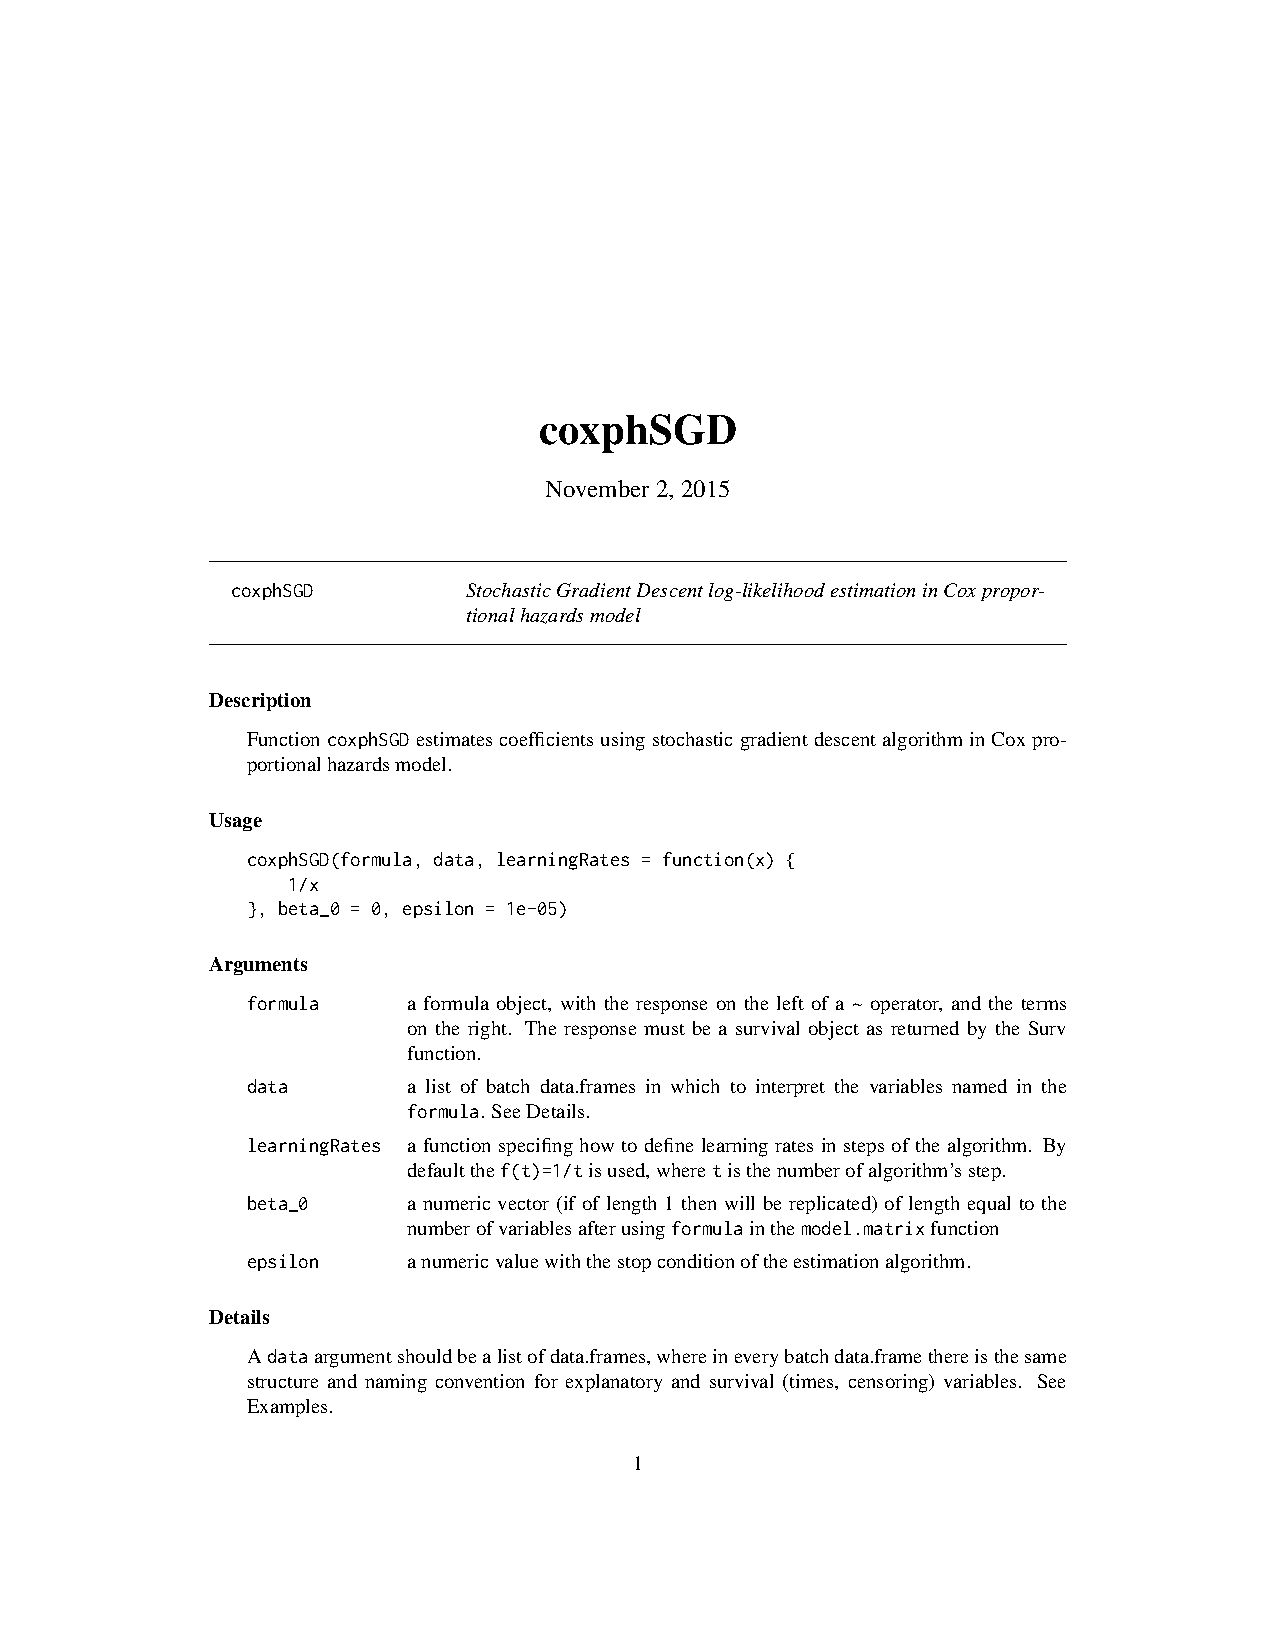
\includepdf[pages=-]{coxphSGD3.pdf}
%\chapter{Dokumentacja pakietu RTCGA}
%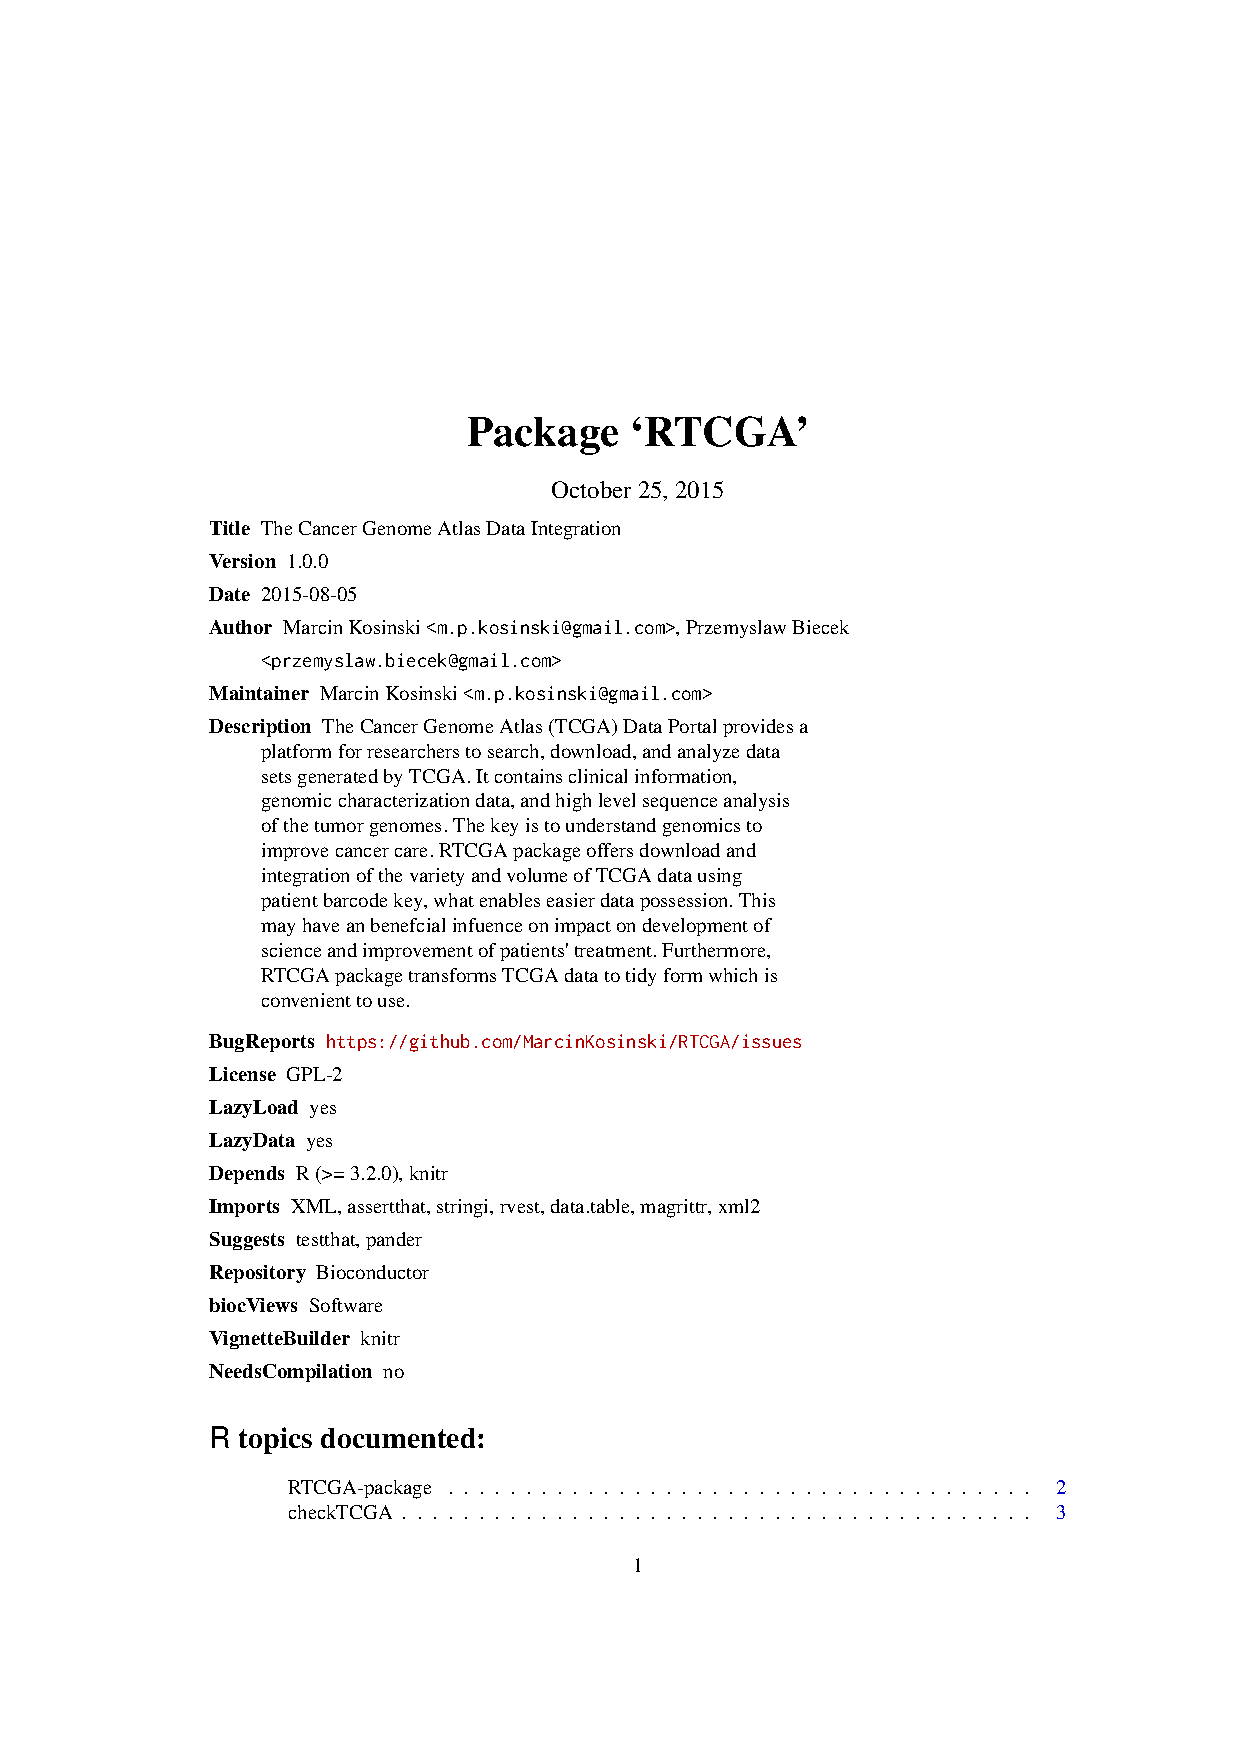
\includepdf[pages=-]{RTCGA.pdf}